\documentclass[10pt,a4paper]{article}
\usepackage[utf8]{inputenc}
\usepackage[francais]{babel}
\usepackage[T1]{fontenc}
\usepackage{listings}
\usepackage{amsmath}
\usepackage{amsfonts}
\usepackage{amssymb}
\usepackage{graphicx}
\author{Gheysen Jeremy, Delgrange Florent}
\title{Réseaux II : TP 1}
\begin{document}
\maketitle

\section{Objectif}

L'objectif de cette séance de travaux pratiques est de se re-familiariser avec les concepts de base des réseaux informatiques comme le fonctionnement de certains services tels DHCP et DNS. Un des buts désirés est aussi d'appréhender de nouveaux concepts plus élaborés comme les protocoles de routage. A cet effet, nous travaillerons avec un ensemble de routeurs CISCO que nous connecterons ensemble selon une topologie bien précise.  

\section{Topologie du réseau mis en place}

Nous disposons pour ce laboratoire du routeur numéro 4, illustré sur la figure \ref{topol} :

\begin{figure}[h]
\begin{center}
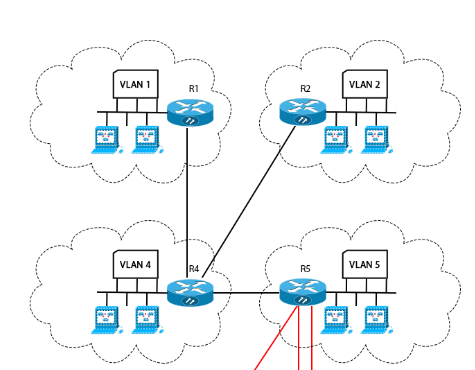
\includegraphics[scale=0.5]{topologie.png}
\caption{Topologie du réseau autour du routeur 4}
\label{topol}
\end{center}
\end{figure}

Nous pouvons remarquer que ce dernier est connecté via ethernet aux routeurs 1,2 et 5 et que le passage par notre routeur est nécessaire pour que la connectivité entre les trois autres routeurs soient établie.

Nous disposions, pour réaliser notre partie de la topologie, d'un routeur CISCO modèle 2600. Ce dernier comporte 4 ports ethernets. Nous avions également à notre disposition 5 ports ethernets d'un switch afin de pouvoir connecter nos machines au sous-réseau.\\
Nous avons donc effectué les connections comme présentées à la figure \ref{topoint}. Nous avons donc relié le port 1/1 du routeur au switch et les autres ports restants aux différents routeurs faisant partie du sous-réseau.  

\begin{figure}[h]
\begin{center}
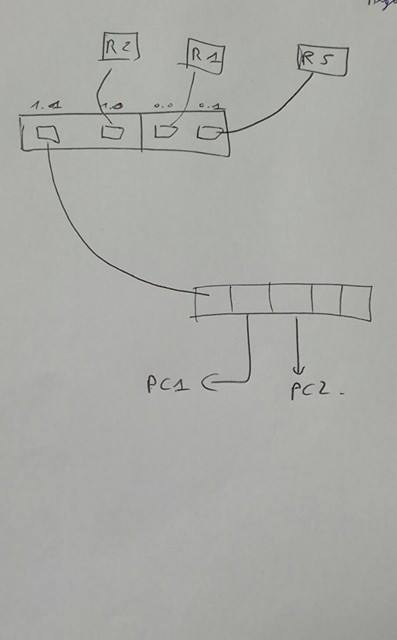
\includegraphics[scale=0.2]{tmp.jpg}
\caption{Sous-réseau attribué au routeur 4}
\label{topoint}
\end{center}
\end{figure}

\section{Description des étapes effectuées}

\noindent Premièrement, on se connecte au routeur numéro 4 :
\begin{lstlisting}[language=bash]
 telnet 192.168.254.144 9004
\end{lstlisting}

\noindent Ensuite, on lance le mode configuration:
\begin{lstlisting}[language=bash]
 enable # acces to more privileges
 conf t # configuration mode; press ctrl z to quit 
\end{lstlisting}

\begin{lstlisting}[language=bash]
 sh int # up or down informations
 sh ip route # show interface route ip attach with the network
\end{lstlisting}

\textit{sh int} Nous indique que la connexion est établie mais qu'aucune interface n'est encore créée (parce que pas encore configurée) et que celui qui est connecté au $5$ est up (car notre routeur est connecté au $5^{eme}$).

\noindent On ouvre les ports ethernets (en étant en \textbf{conf t})
\begin{lstlisting}[language=bash]
int ethernet 0/0 # we acces to ethernet 0/0 port
no shutdown # up the ethernet port
\end{lstlisting}

On connecte maintenant le routeur au switch sur l'interface ethernet 1/1. On attribue maintenant une adresse à l'interface du routeur.

\noindent On attribue une adresse IP à l'interface.
\begin{lstlisting}[language=bash]
conf t
int ethernet 1/1
ip address 192.168.104.002 255.255.255.248
\end{lstlisting}
\textbf{Pourquoi 3 bits ?}\\
Le 1er bit réservé (1 pour le broadcast 0 pour la machine). On a 4 ports de disponibles.\\
On configure par la suite toutes les interfaces de cette façon.

\subsection{Le DHCP}

\noindent On configure le DHCP
\begin{lstlisting}[language=bash]
ip dhcp pool giorgio
network 192.168.104.0 255.255.255.248
dns-server 192.168.104.0
default-router 192.168.104.0
lease 5 0 0
\end{lstlisting}

En tentant de connecter un PC, celui-ci obtient bien une adresse depuis le routeur, on peut la récupérer grace à la commande \textbf{ifconfig} : 192.168.104.7 \\
Si on ping le routeur, celui-ci répond également positivement avec 

\noindent ping
\begin{lstlisting}[language=bash]
ping 192.168.104.2
PING 192.168.104.2 (192.168.104.2): 56 data bytes
64 bytes from 192.168.104.2: icmp_seq=0 ttl=255 time=2.050 ms
64 bytes from 192.168.104.2: icmp_seq=2 ttl=255 time=2.076 ms
64 bytes from 192.168.104.2: icmp_seq=3 ttl=255 time=2.062 ms
64 bytes from 192.168.104.2: icmp_seq=4 ttl=255 time=2.311 ms
...
\end{lstlisting}
show ip DHCP pool

\noindent Connexion avec le routeur 5
\begin{lstlisting}[language=bash]
int ethernet 0/1
ip adress 192.168.142.2 255.255.255.248
\end{lstlisting}

\subsection{OSPF}

\noindent Configuration OSPF
\begin{lstlisting}[language=bash]
conf t
router ospf 10
newtork 192.168.104.0 0.0.0.255 area 0
\end{lstlisting}
\end{document}